\subsection*{Problem 4: LQR State Feedback Regulation}

The following table outlines the 5 different combinations of $Q$ and $R$ with the corresponding $K$ we tested on the linear model. The values for $Q$ in the table indicate the diagonal terms with the off-diagonal terms being 0. The $Q$ for Combination 1 was derived using $Q = C^TQ_1C$.

\begin{table}[!ht]
    \centering
    \caption{Q $\&$ R Combinations with Resulting K $\&$ s}
    \begin{tabular}{|*5{c|}}
        \hline
        $\#$ & $Q$                                                                           & $R$ & $K$                                                           & $s$                                                             \\ [0.5ex]
        \hline
        1    & $diag\left(\begin{bmatrix}3.31 \\ 0  \\ 2.69 \\ 0 \end{bmatrix}\right)$       & 1   & $\begin{bmatrix} -1.82 & -2.38 & 20.85 & 3.89 \end{bmatrix}$  & $\begin{array}{cc} -1.14\pm1.11 \\ -5.62\pm0.67 \end{array}$    \\
        \hline
        2    & $diag\left(\begin{bmatrix}33.06 \\ 10  \\ 26.87 \\ 10 \end{bmatrix}\right)$   & 1   & $\begin{bmatrix} -5.75 & -6.92 & 38.02  & 7.96 \end{bmatrix}$ & $\begin{array}{cc} -1.96 \\ -2.37\pm1.44 \\  -17.07\end{array}$ \\
        \hline
        3    & $diag\left(\begin{bmatrix}3.31 \\ 1  \\ 2.69 \\ 1 \end{bmatrix}\right)$       & 10  & $\begin{bmatrix} -0.58 & -1.27 & 17.57 & 3.25 \end{bmatrix}$  & $\begin{array}{cc} -0.68\pm0.59 \\ -4.95 \\  -6.33\end{array}$  \\
        \hline
        4    & $diag\left(\begin{bmatrix}3.31 \\ 1  \\ 2.69 \\ 1 \end{bmatrix}\right)$       & 1   & $\begin{bmatrix} -1.82 & -2.70 & 22.32 & 4.30  \end{bmatrix}$ & $\begin{array}{cc} -1.32\pm0.88 \\  -3.85 \\ -8.34\end{array}$  \\
        \hline
        5    & $diag\left(\begin{bmatrix}0.17 \\ 0.05  \\ 0.13 \\ 0.05 \end{bmatrix}\right)$ & 1   & $\begin{bmatrix} -0.41 & -1.04 & 16.84 & 3.10  \end{bmatrix}$ & $\begin{array}{cc} -0.57\pm0.51 \\  -5.13 \\ -6.10\end{array}$  \\
        \hline
    \end{tabular}
\end{table}

\clearpage

The following figures depict the outputs and input of the linear system with the above controllers from the 5 combinations:

\begin{figure}[!ht]
    \centering
    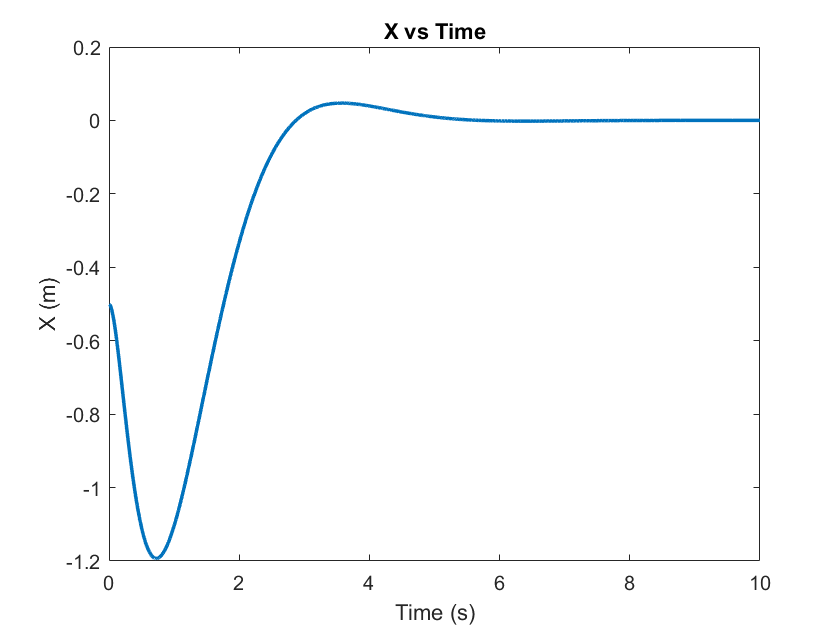
\includegraphics[width=\linewidth]{figs/sf_lin_c1_x.png}
    \caption{Combination $\#$1 - Linear System X Output}
    \label{}
\end{figure}

\begin{figure}[!ht]
    \centering
    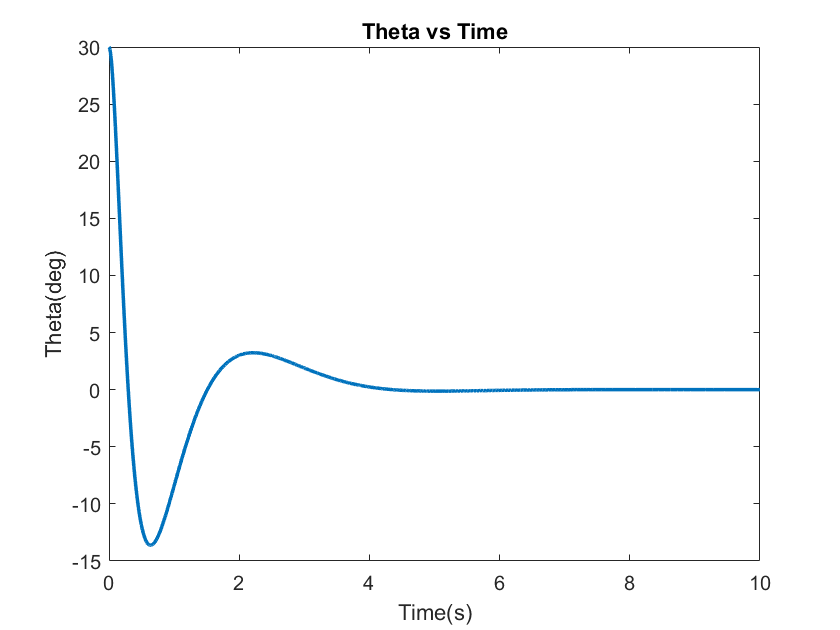
\includegraphics[width=\linewidth]{figs/sf_lin_c1_theta.png}
    \caption{Combination $\#$1 - Linear System $\theta$ Output}
    \label{}
\end{figure}

\begin{figure}[!ht]
    \centering
    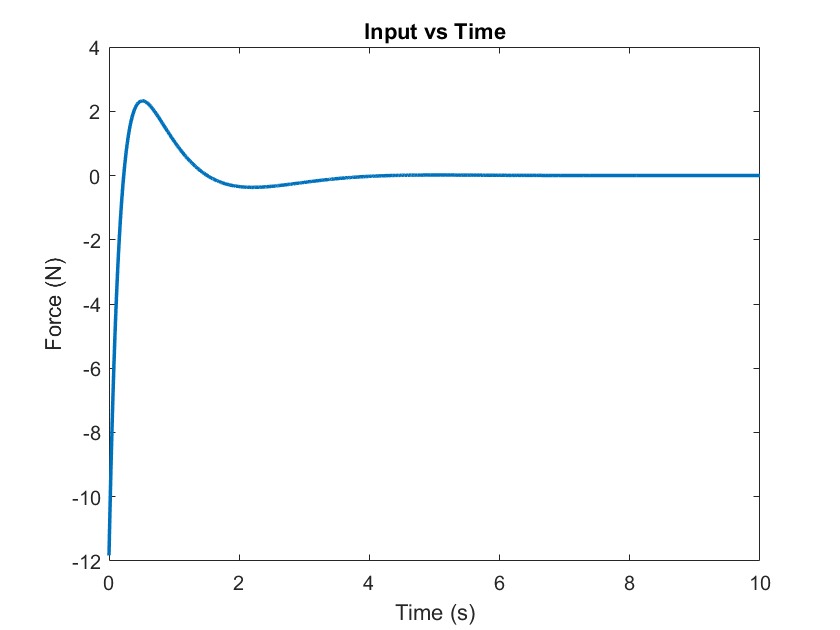
\includegraphics[width=\linewidth]{figs/sf_lin_c1_input.png}
    \caption{Combination $\#$1 - Linear System Input}
    \label{}
\end{figure}

\begin{figure}[!ht]
    \centering
    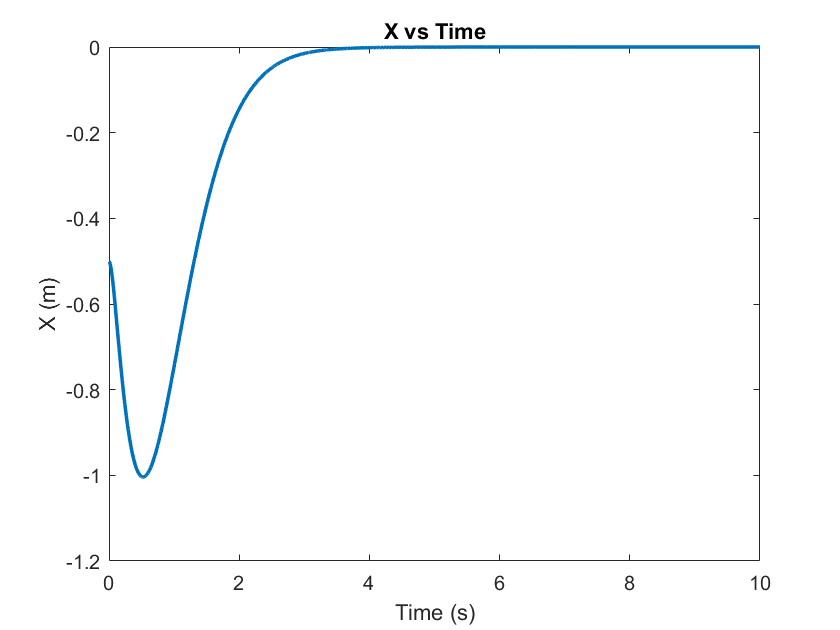
\includegraphics[width=\linewidth]{figs/sf_lin_c2_x.png}
    \caption{Combination $\#$2 - Linear System X Output}
    \label{}
\end{figure}

\begin{figure}[!ht]
    \centering
    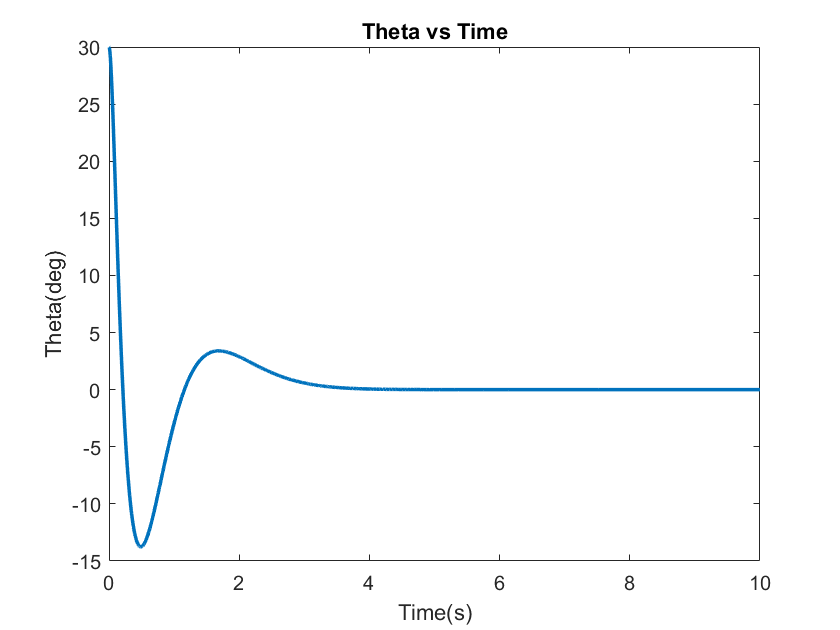
\includegraphics[width=\linewidth]{figs/sf_lin_c2_theta.png}
    \caption{Combination $\#$2 - Linear System $\theta$ Output}
    \label{}
\end{figure}

\begin{figure}[!ht]
    \centering
    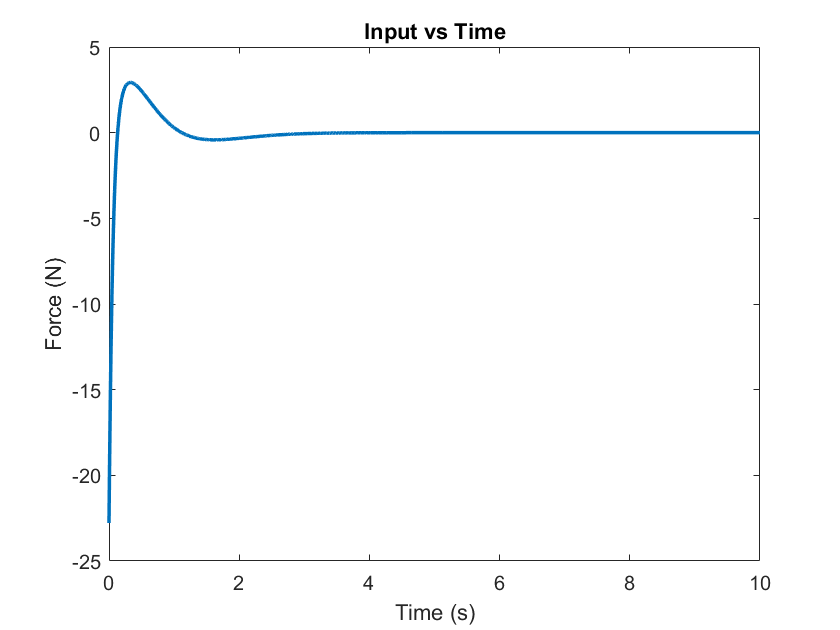
\includegraphics[width=\linewidth]{figs/sf_lin_c2_input.png}
    \caption{Combination $\#$2 - Linear System Input}
    \label{}
\end{figure}

\begin{figure}[!ht]
    \centering
    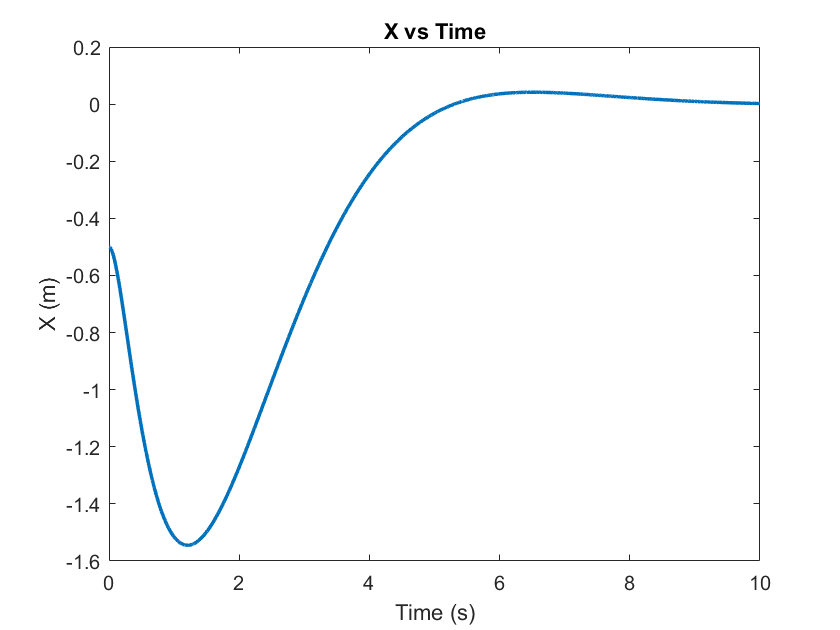
\includegraphics[width=\linewidth]{figs/sf_lin_c3_x.png}
    \caption{Combination $\#$3 - Linear System X Output}
    \label{}
\end{figure}

\begin{figure}[!ht]
    \centering
    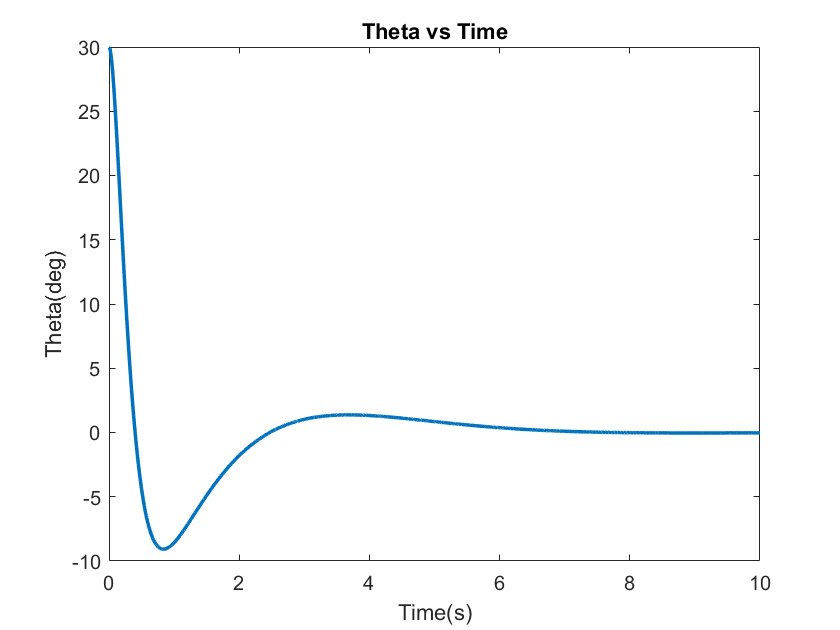
\includegraphics[width=\linewidth]{figs/sf_lin_c3_theta.png}
    \caption{Combination $\#$3 - Linear System $\theta$ Output}
    \label{}
\end{figure}

\begin{figure}[!ht]
    \centering
    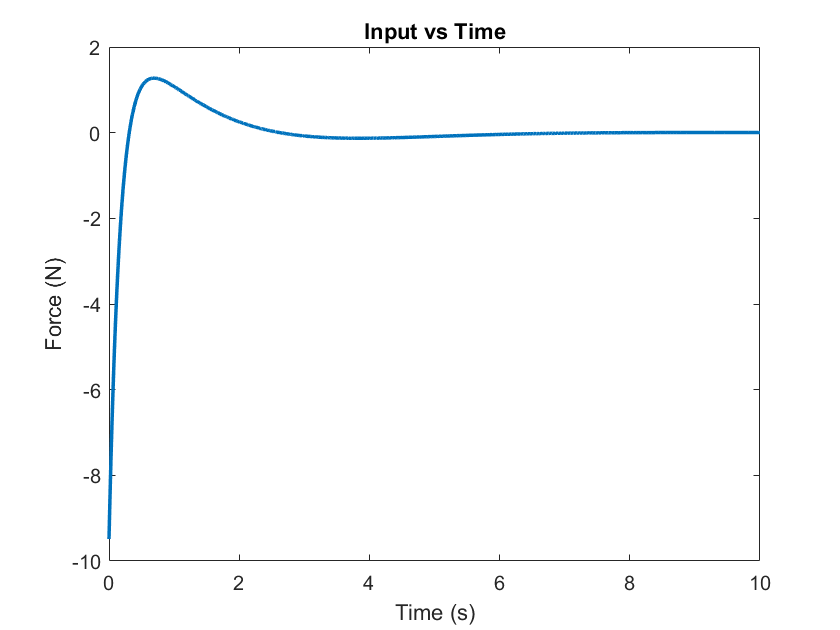
\includegraphics[width=\linewidth]{figs/sf_lin_c3_input.png}
    \caption{Combination $\#$3 - Linear System Input}
    \label{}
\end{figure}

\begin{figure}[!ht]
    \centering
    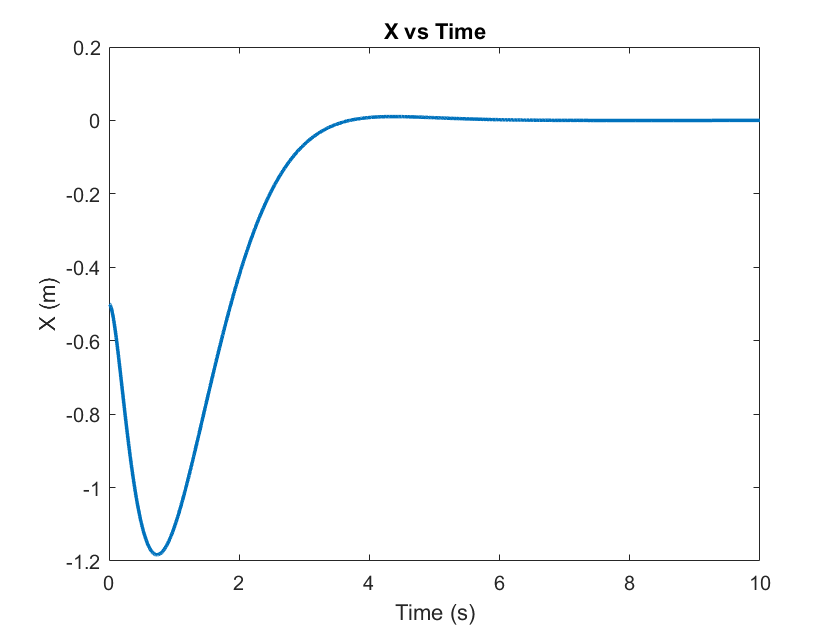
\includegraphics[width=\linewidth]{figs/sf_lin_x.png}
    \caption{Combination $\#$4 - Linear System X Output}
    \label{}
\end{figure}

\begin{figure}[!ht]
    \centering
    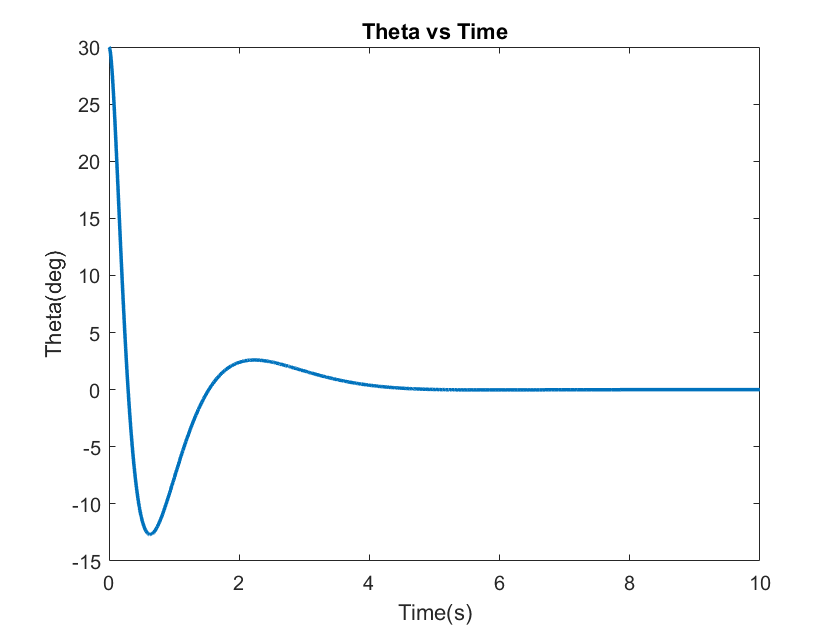
\includegraphics[width=\linewidth]{figs/sf_lin_theta.png}
    \caption{Combination $\#$4 - Linear System $\theta$ Output}
    \label{}
\end{figure}

\begin{figure}[!ht]
    \centering
    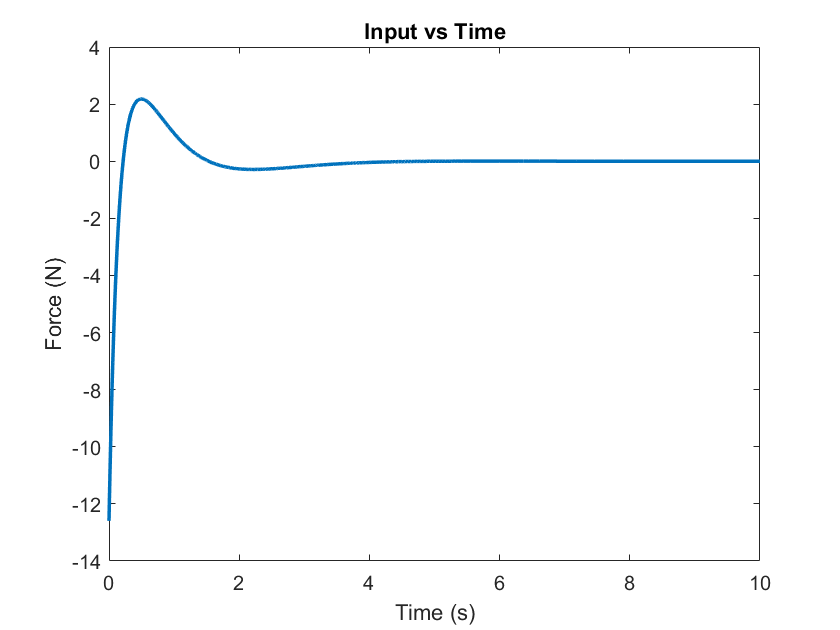
\includegraphics[width=\linewidth]{figs/sf_lin_input.png}
    \caption{Combination $\#$4 - Linear System Input}
    \label{}
\end{figure}

\begin{figure}[!ht]
    \centering
    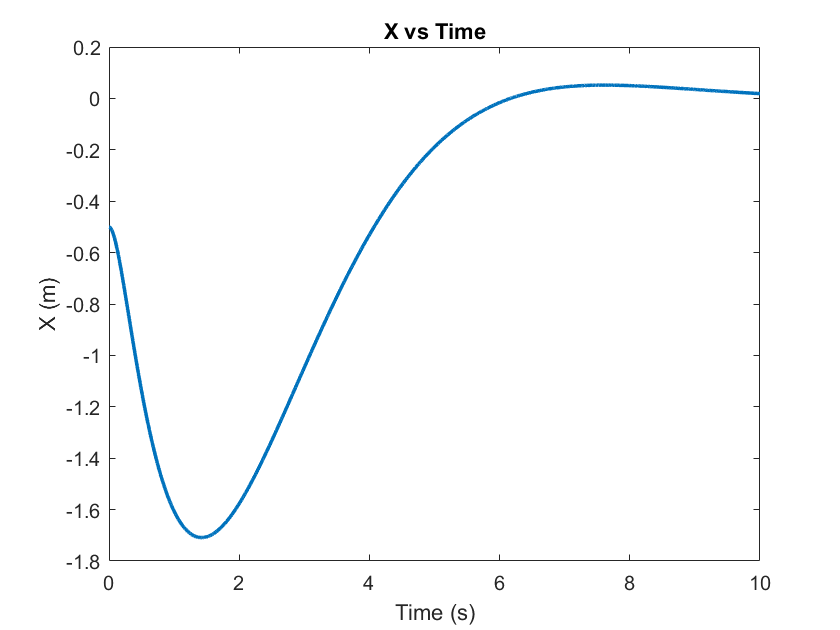
\includegraphics[width=\linewidth]{figs/sf_lin_c5_x.png}
    \caption{Combination $\#$5 - Linear System X Output}
    \label{}
\end{figure}

\begin{figure}[!ht]
    \centering
    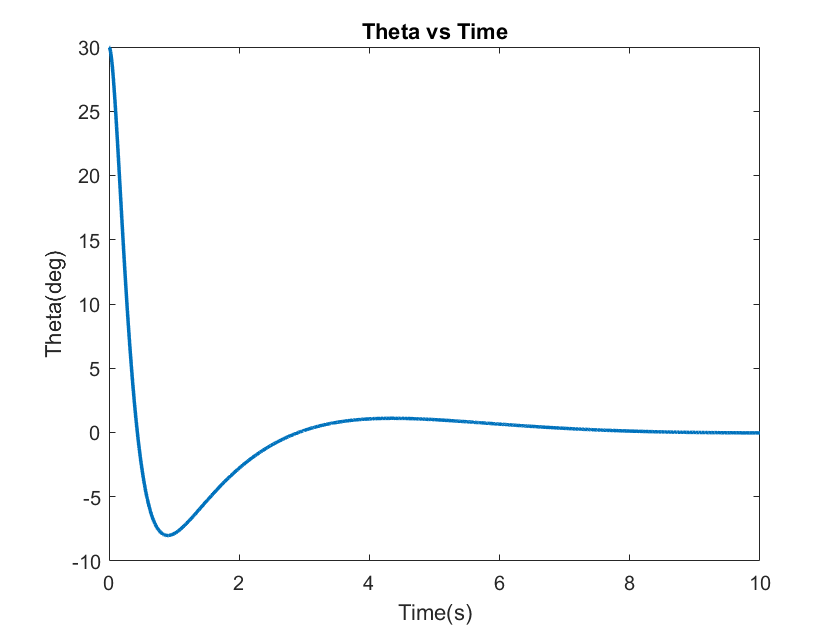
\includegraphics[width=\linewidth]{figs/sf_lin_c5_theta.png}
    \caption{Combination $\#$5 - Linear System $\theta$ Output}
    \label{}
\end{figure}

\begin{figure}[!ht]
    \centering
    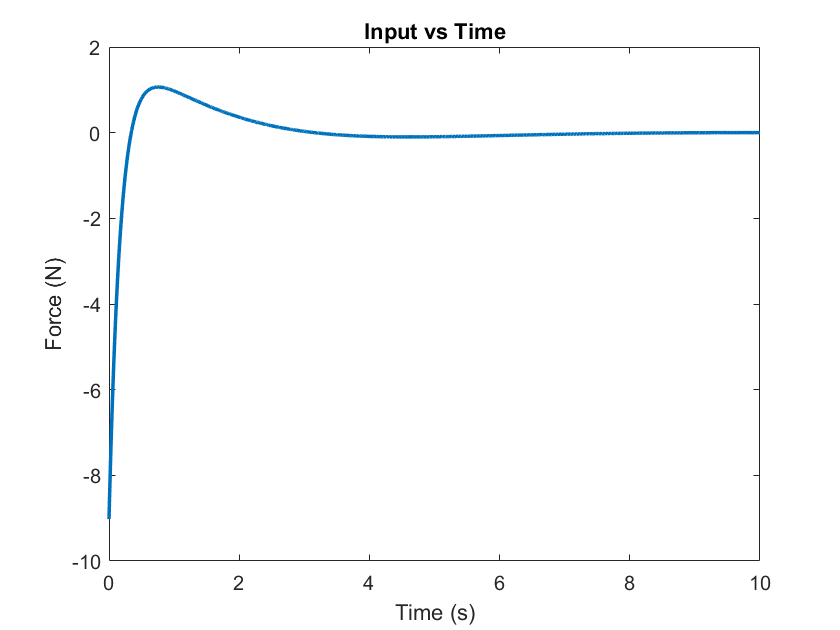
\includegraphics[width=\linewidth]{figs/sf_lin_c5_input.png}
    \caption{Combination $\#$5 - Linear System Input}
    \label{}
\end{figure}

\clearpage


Overall, increasing the values of $Q$ made the state response quicker without drastically changing the input (however it slightly increases) and decreasing $Q$ makes the response slower, but doesn't drastically change the input.  On the other hand, increasing $R$ decreased the input and made the response slower. Decreasing $R$ did the opposite. Using the modified $Q$ in Combination 1 eliminates the consideration for the derivative states which makes the response slightly slower while still being somewhat similar.